%%% Template originaly created by Karol Kozioł (mail@karol-koziol.net) and modified for ShareLaTeX use

\documentclass[a4paper,11pt]{article}

\usepackage{indentfirst}
\usepackage[T1]{fontenc}
\usepackage[utf8]{inputenc}
\usepackage{graphicx}
\graphicspath{ {./images/} }

\usepackage{xcolor}

\renewcommand\familydefault{\sfdefault}
\usepackage{tgheros}

\usepackage{amsmath,amssymb,amsthm,textcomp,latexsym}
\usepackage{enumerate}
\usepackage{multicol}
\usepackage{tikz}

\usepackage{caption}
\usepackage{subcaption}
\usepackage{epstopdf}
\usepackage{cancel}
\usepackage{mathtools}


\usepackage{geometry}
\geometry{total={210mm,297mm},
left=25mm,right=25mm,%
bindingoffset=0mm, top=20mm,bottom=20mm}


\linespread{1.3}

\newcommand{\linia}{\rule{\linewidth}{0.5pt}}

% custom theorems if needed
\newtheoremstyle{mytheor}
    {1ex}{1ex}{\normalfont}{0pt}{\scshape}{.}{1ex}
    {{\thmname{#1 }}{\thmnumber{#2}}{\thmnote{ (#3)}}}

\theoremstyle{mytheor}
\newtheorem{defi}{Definition}

% my own titles
\makeatletter
\renewcommand{\maketitle}{
\begin{center}
\vspace{2ex}
{\huge \textsc{\@title}}
\vspace{1ex}
\\
\linia\\
\@author \hfill \@date
\vspace{4ex}
\end{center}
}
\makeatother
%%%

% custom footers and headers
\usepackage{fancyhdr}
\pagestyle{fancy}
\lhead{Projeto 2}
\chead{}
\rhead{2019.2}
\lfoot{}
\cfoot{}
\rfoot{Page \thepage}
\renewcommand{\headrulewidth}{0pt}
\renewcommand{\footrulewidth}{0pt}
%

% code listing settings
\usepackage{listings}
\lstset{
    language=Matlab,
    basicstyle=\ttfamily\small,
    aboveskip={1.0\baselineskip},
    belowskip={1.0\baselineskip},
    columns=fixed,
    extendedchars=true,
    breaklines=true,
    tabsize=4,
    prebreak=\raisebox{0ex}[0ex][0ex]{\ensuremath{\hookleftarrow}},
    frame=lines,
    showtabs=false,
    showspaces=false,
    showstringspaces=false,
    keywordstyle=\color[rgb]{0.627,0.126,0.941},
    commentstyle=\color[rgb]{0.133,0.545,0.133},
    stringstyle=\color[rgb]{01,0,0},
    numbers=left,
    numberstyle=\small,
    stepnumber=1,
    numbersep=10pt,
    captionpos=t,
    escapeinside={\%*}{*)}
}

%%%----------%%%----------%%%----------%%%----------%%%


\DeclarePairedDelimiter\abs{\lvert}{\rvert}%
\DeclarePairedDelimiter\norm{\lVert}{\rVert}%

% Swap the definition of \abs* and \norm*, so that \abs
% and \norm resizes the size of the brackets, and the 
% starred version does not.
\makeatletter
\let\oldabs\abs
\def\abs{\@ifstar{\oldabs}{\oldabs*}}
%
\let\oldnorm\norm
\def\norm{\@ifstar{\oldnorm}{\oldnorm*}}
\makeatother

\begin{document}

\title{Robótica e Automação}

\author{Raphael Barros Parreira}

\date{}

\maketitle

\section{Controle Cinemático de Manipuladores} % 1

O exercício tem como objetivo o \textbf{controle cinemático} da posição do punho do manipulador, sem se preocupar com a orientação, nesse primeiro momento. Para isso, o manipulador escolhido foi um 7R, com a tabela de Denavit-Hartenberg (tabela \ref{tab:ex1_dh}) e a posição inicial ($q_0$ representada na figura \ref{fig:ex1_ready}) dadas.

Além disso, o enunciado define 3 trajetórias distintas, define os controles a serem implementados e insere restrições.

Como o objetivo é apenas controlar a posição do manipulador, pode-se ignorar as 3 últimas juntas, já que, pela tabela de DH, elas apenas influenciam na orientação do manipulador. Essa decisão implicará numa série de simplificações feitas no sistema, começando por sempre definir a posição e a velocidade dessas 3 juntas como $zero$.


\begin{figure}[!ht]
\centering
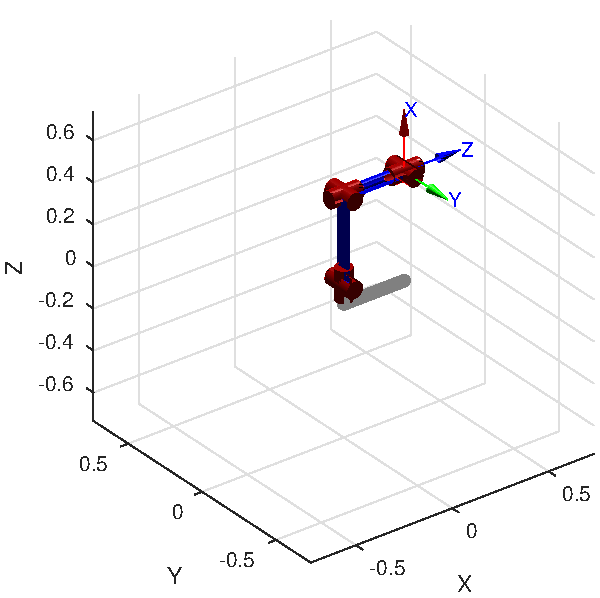
\includegraphics[width=0.5\textwidth]{figs/ex1_ready.pdf}
\caption{Manipulador Antropomórfico na posição inicial}
\label{fig:ex1_ready}
\end{figure}

\begin{gather*}
\theta_5 = \theta_6 = \theta_7 = 0 \\
\dot{\theta_5} = \dot{\theta_6} = \dot{\theta_7} = 0 \\
q_0 = [0, 0, 0, \pi/2] \\
\dot{\theta}_{max} = 3 rad/s \Rightarrow \norm{u_i} \leq 3 (i = 1,2,3)
\end{gather*}

\begin{table}[!ht]
\centering
\caption{Tabela de Denavit-Hartenberg do Manipulador Antropomórfico.}
\label{tab:ex1_dh}

\begin{tabular}{|c|c|c|c|c|c|}
\hline
Junta  & $\alpha (rad)$ & $A (m)$ & $\theta (rad)$ & $D (m)$ & $Offset (rad)$ \\ \hline
$1$  & $\pi/2$ & 0 & $\theta_1$ & 0 & 0 \\ \hline
$2$  & $\pi/2$ & 0 & $\theta_2$ & 0 & $\pi$ \\ \hline
$3$  & $\pi/2$ & 0 & $\theta_3$ & $-0.4208$ & $\pi$ \\ \hline
$4$  & $\pi/2$ & 0 & $\theta_4$ & 0 & $\pi$ \\ \hline
$5$  & $\pi/2$ & 0 & $\theta_5$ & $-0.3143$ & $\pi$ \\ \hline
$6$  & $\pi/2$ & 0 & $\theta_6$ & 0 & $\pi$ \\ \hline
$7$  & $\pi$   & 0 & $\theta_7$ & 0 & $\pi$ \\ \hline

\end{tabular}
\end{table}

\subsection{Controle}


No controle cinemático assume-se que a velocidade do manipulador é a variável manipulada e que a \textbf{dinâmica} do manipulador pode ser \textbf{desprezada}. Além disso, considera-se que a velocidade das juntas responde instantaneamente ao sinal de entrada do motor da mesma, implicando na condição de $ u \approx \dot{\theta} $

\begin{gather*}
\begin{bmatrix} \vec{v} \\ \vec{\omega} \end{bmatrix} = J(\theta)\dot{\theta} \quad \Rightarrow \quad  \begin{bmatrix} \vec{v} \\ \vec{\omega} \end{bmatrix} = J(\theta)u\\
u = \dot{\theta} \quad \Rightarrow \quad \dot{x} = J(\theta)u \\
x(t) \longrightarrow x_d(t) \\
e = x - x_d \\
\end{gather*}

O objetivo de controle é que o manipulador siga uma trajetória pré-determinada. Portanto, já que se conhece a trajetória, por conseguinte, também se conhece a sua derivada. O que permite adicionar informações no sistema de controle (ação \textit{feed-forward}, tornando possível a \textbf{liminação do erro em estado estacionário} ao seguir uma trajetória.

Para que os cálculos sejam feitos, é necessário escolher uma base para expressar os vetores e calcular o Jacobiano. Já que a trajetória dada está expressa na base do sistema inercial, uma boa escolha é usar essa mesma base.

Uma boa ideia para a lei de controle é eliminar as não-linearidades do sistema, incluindo-se a inversa do Jacobiano no sinal de controle.

\begin{gather*}
\dot{x} = J\bar{u} \\
\bar{u} = J^{-1} [ \dot{x_d} + K (x_d - x) ] \\
\dot{x} = JJ^{-1} [ \dot{x_d} + K (x_d - x) ] \\
\dot{x} - \dot{x_d} = K (x_d - x) \\
\dot{e}(t)= Ke(t)  \\
e \longrightarrow 0, \quad t \longrightarrow \infty
\end{gather*}

Como no caso de um manipulador com 7 juntas, o Jacobiano não é uma matriz quadrada, ele não possui inversa. Sendo assim, se faz necessário o uso da \textbf{pseudo-inversa} ($ J^\dagger $).


\begin{gather*}
J^\dagger = J^T(JJ^T)^{-1} \quad \Rightarrow \quad JJ^\dagger = I \\
\bar{u} = J^{\dagger} [ \dot{x_d} + K (x_d - x) ] \\
\end{gather*}


\subsection{Trajetórias}

O enunciado considera 3 trajetórias de referência distintas, com $w_n = 2\pi/10 $. Além disso, não se pode usar derivadores puros. Logo, as derivadas das trajetórias foram calculadas como se segue:

\renewcommand{\labelenumi}{\alph{enumi}}
 \begin{enumerate}
   \item Trajetória a
   	\begin{gather*}
	x_{d} = 
	\begin{bmatrix} 
	0.075 (sin(w_n t) + sin( 4 w_n t)) + 0.456 \\ 
	0 \\ 
	0.075 (cos(w_n t) + cos( 4 w_n t)) + 0.069 
	\end{bmatrix} \\
	\dot{x_{d}} = 
	\begin{bmatrix}
	0.075 w_n (cos(w_n t) + 4 cos( 4 w_n t)) \\ 
	0 \\ 
	-0.075 w_n (sin(w_n t) + 4 sin( 4 w_n t)) 
	\end{bmatrix} \\
	\end{gather*}
   \item Trejetória b
   	\begin{gather*}
	x_{d} = 
	\begin{bmatrix} 
	0.075 sin(w_n t) + 0.456 \\ 
	0 \\ 
	0.075 cos(w_n t) + 0.2 
	\end{bmatrix} \\
	\dot{x_{d}} = 
	\begin{bmatrix} 
	0.075 w_n cos(w_n t) \\ 
	0 \\ 
	- 0.075 w_n sin(w_n t) 
	\end{bmatrix} \\
	\end{gather*}
   \item Trejetória c
   	\begin{gather*}
	x_{d} = 
	\begin{bmatrix} 
	0.075 sin(w_n t) + 0.456 \\ 
	0.075 (sin(w_n t) + cos(w_n t)) \\ 
	0.075 cos(w_n t) + 0.2 
	\end{bmatrix} \\
	\dot{x_{d}} = 
	\begin{bmatrix} 
	0.075 w_n cos(w_n t) \\ 
	0.075 w_n (sin(w_n t) - sin(w_n t)) \\ 
	- 0.075 w_n sin(w_n t) 
	\end{bmatrix} \\
	\end{gather*}
 \end{enumerate}


\subsection{Simulação}

O sistema representado na topologia da figura \ref{fig:ex1_simulink} está simulando a lei de controle com o feed-forward. Porém, para efeitos de comparação, o exercício pede para desligar essa ação. Para isso, basta apenas excluir o sinal de $xddot$ que é somado depois do ganho.

Cada uma das trajetórias foi simulada com e sem ação do feed-forward.

\begin{figure}[!ht]
\centering
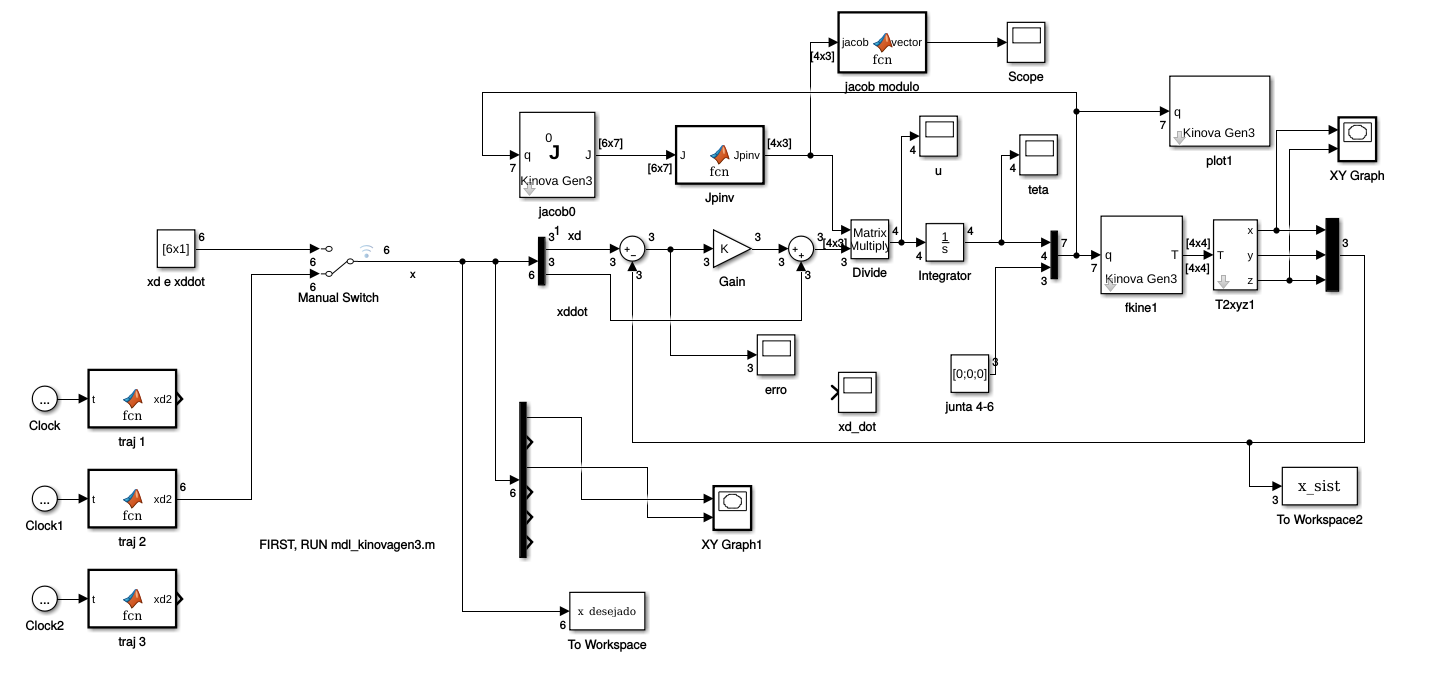
\includegraphics[width=1\textwidth]{figs/ex1_simulink}
\caption{Topologia do Simulink.}
\label{fig:ex1_simulink}
\end{figure}


\subsection{Ganhos}

Um ponto importante do trabalho é o ganho $K$ do controlador. Isso se dá porque foi pedido o maior ganho possível atendendo à especificação de $ \norm{u_i} \leq 3 (i = 1,2,3)$.

Sendo assim, se faz necessário calcular a ordem de grandeza do ganho e depois se fazer o ajuste fino para cada um dos casos.

\begin{gather*}
\norm{\bar{u}} \leq 3 \quad \Rightarrow \quad \norm{J^{\dagger} [ \dot{x_d} + K (x_d - x) ]} \leq 3 \\
\norm{J^{\dagger}}_{max} [ \norm{\dot{x_d}}_{max} + K_{base} \norm{e}_{max} ] = 3\\
K_{base} = \dfrac{\dfrac{3}{\norm{J^\dagger}_{max}} - \norm{\dot{x}_d}_{max}}{\norm{e}_{max}} \\
\norm{J^\dagger}_{max} = 4.277 \qquad
\norm{\dot{x}_d}_{max} = 0.2356 \qquad
\norm{e}_{max} = 0.1417 \\
K_{base} \approx 3.3
\end{gather*}

Os valores $ \norm{J^\dagger}_{max} $, $ \norm{\dot{x}_d}_{max} $ e $ \norm{e}_{max} $ foram calculados graficamente na simulação, considerando o valor no instante inicial ($ \theta(0) $), onde se mostrou ser o maior valor em todos os casos.

Após esse passo, foi feita a sintonia fina, chegando o mais próximo possível do valor máximo do sinal de controle em cada um dos casos. Os valores encontrados podem ser vistos na tabela \ref{tab:ex1_ganhos}.

\begin{table}[!ht]
\centering
\caption{Ganhos para os controles com e sem Feed-forward em todas as 3 trajetórias.}
\label{tab:ex1_ganhos}

\begin{tabular}{|c|c|c|}
\hline
Controles  & FB & FF \\ \hline
Trajetória 1     & $8.91$ & $7.24$ \\ \hline
Trajetória 2     & $8.91$ & $8.57$ \\ \hline
Trajetória 3     & $8.91$ & $8.57$ \\ \hline
\end{tabular}
\end{table}


\subsection{Resultados}

Cada uma das trajetórias tem dois conjuntos de figuras representando os dois controles pedidos (com e sem feed-forward). 

Desses conjuntos, a figura (a) exibe a trajetórias desejada (em vermelho) e a trajetória simulada (em azul). A figura (b), por sua vez, exibe o sinal do erro ($x_d - x$). Já a figura (c) representa o sinal de controle $u$ para cada uma das 4 juntas controladas.

Como esperado, o controle sem feed-forward não é capaz de tirar o erro em regime de estado estacionário, mesmo sendo muito pequeno. Os sinais de controle atendem à restrição pedida, sempre se aproximando o máximo possível do valor máximo.

Pode-se observar na tabela \ref{tab:ex1_ganhos} que os ganhos para o controle sem ação feed-forward são iguais para todas as trajetórias, sendo limitado apenas pela restrição do sinal de controle. Porém, mesmo aumentando o valor do ganho não seria possível eliminar o erro em EE.

No caso de não ser possível calcular a derivada da trajetória e, dependendo do caso de aplicação do manipulador, o controlador apenas com feed-back de posição pode ser suficiente, já que o erro em EE é pequeno comparado ao tamanho dos elos.


\begin{figure}[!ht]
\centering
  \begin{minipage}{\linewidth}
  \centering
    \begin{subfigure}[b]{0.4\textwidth}
    		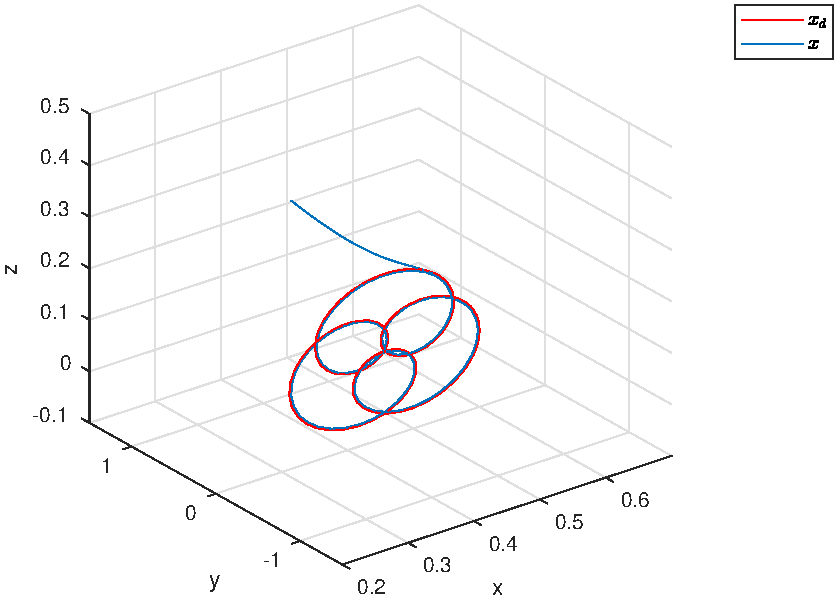
\includegraphics[width=1\textwidth]{figs/ex1_a_2_x.pdf}
    		\caption{$x_d$ e $x$}
    		\label{fig:ex1_a_2_x}
    \end{subfigure}
  \end{minipage}
  \begin{minipage}{\linewidth}
  \centering
    \begin{subfigure}[b]{0.4\textwidth}
    		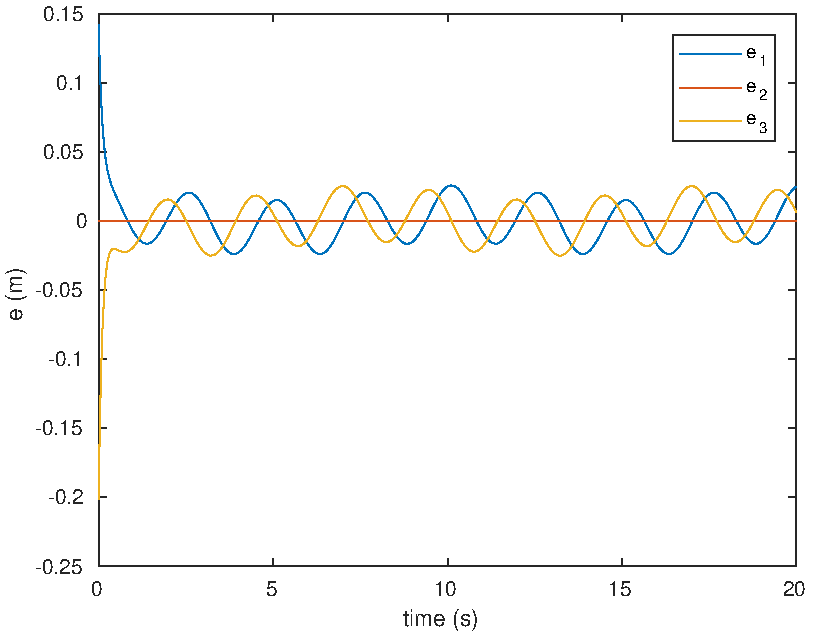
\includegraphics[width=1\textwidth]{figs/ex1_a_2_e.pdf}
    		\caption{$e = x_d - x$}
    		\label{fig:ex1_a_2_e}
    \end{subfigure}
    \begin{subfigure}[b]{0.4\textwidth}
    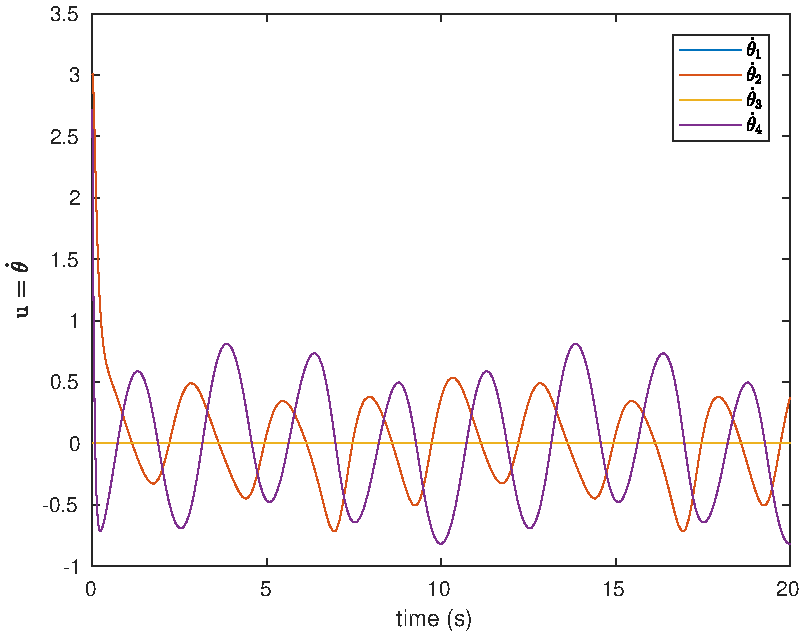
\includegraphics[width=1\textwidth]{figs/ex1_a_2_dq.pdf}
    \caption{$u = \dot{\theta}$}
    \label{fig:ex1_a_2_dq}
    \end{subfigure}
  \end{minipage}
\caption{Ex 1: Trajetória $a$, controle sem FF.}
\label{fig:ex1_a_2}
\end{figure}

\begin{figure}[!ht]
\centering
  \begin{minipage}{\linewidth}
  \centering
    \begin{subfigure}[b]{0.4\textwidth}
    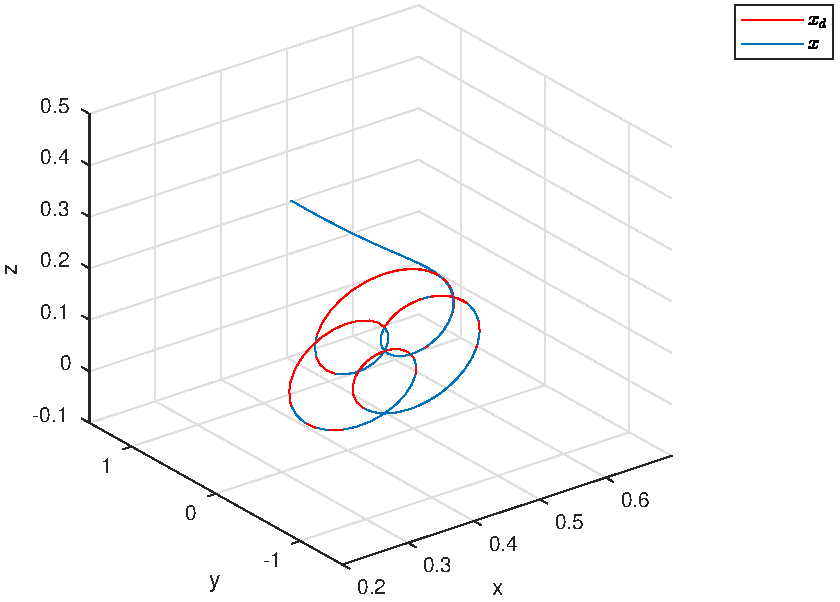
\includegraphics[width=1\textwidth]{figs/ex1_a_1_x.pdf}
    \caption{$x_d$ e $x$}
    \label{fig:ex1_a_1_x}
    \end{subfigure}
  \end{minipage}
  \begin{minipage}{\linewidth}
  \centering
    \begin{subfigure}[b]{0.4\textwidth}
    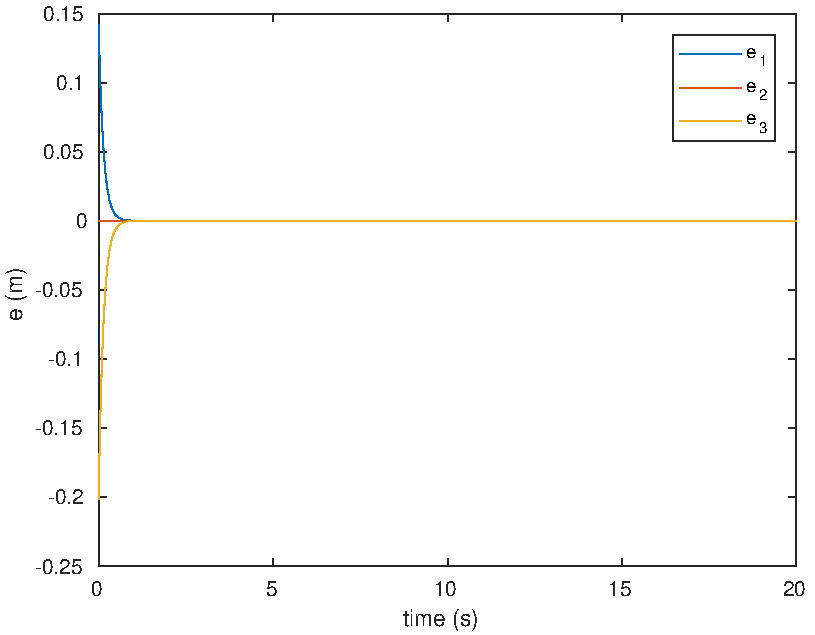
\includegraphics[width=1\textwidth]{figs/ex1_a_1_e.pdf}
    \caption{$e = x_d - x$}
    \label{fig:ex1_a_1_e}
    \end{subfigure}
    \begin{subfigure}[b]{0.4\textwidth}
    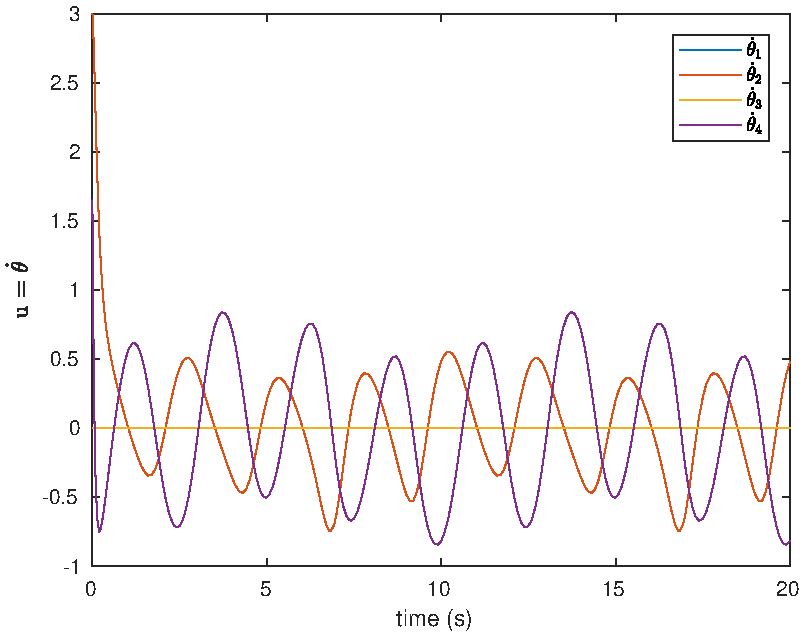
\includegraphics[width=1\textwidth]{figs/ex1_a_1_dq.pdf}
    \caption{$u = \dot{\theta}$}
    \label{fig:ex1_a_1_dq}
    \end{subfigure}
  \end{minipage}
\caption{Ex 1: Trajetória $a$, controle com FF.}
\label{fig:ex1_a_1}
\end{figure}


\begin{figure}[!ht]
\centering
  \begin{minipage}{\linewidth}
  \centering
    \begin{subfigure}[b]{0.4\textwidth}
    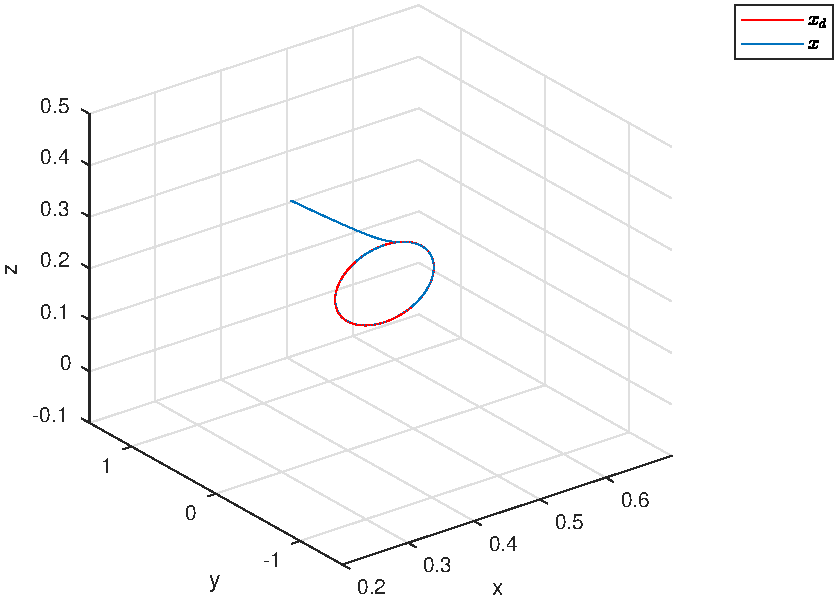
\includegraphics[width=1\textwidth]{figs/ex1_b_2_x.pdf}
    \caption{$x_d$ e $x$}
    \label{fig:ex1_b_2_x}
    \end{subfigure}
  \end{minipage}
  \begin{minipage}{\linewidth}
  \centering
    \begin{subfigure}[b]{0.4\textwidth}
    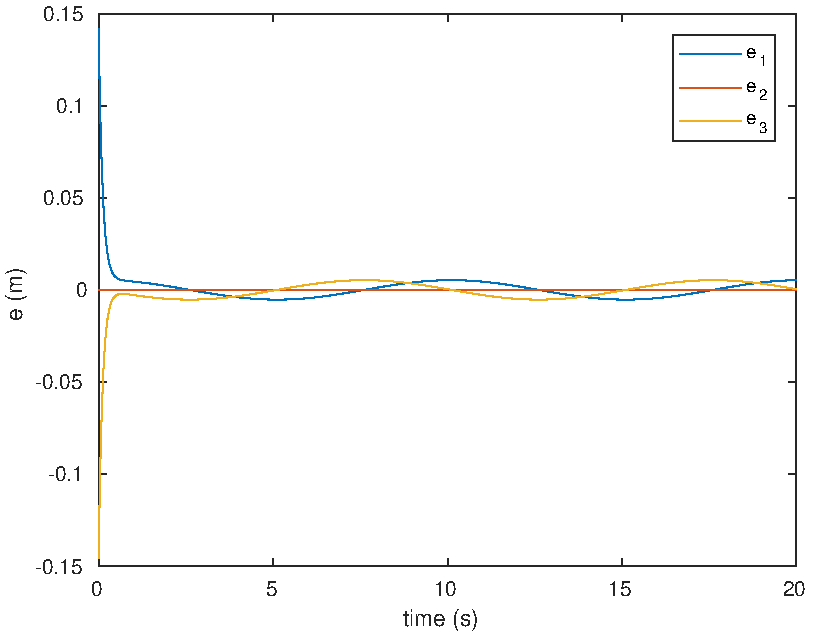
\includegraphics[width=1\textwidth]{figs/ex1_b_2_e.pdf}
    \caption{$e = x_d - x$}
    \label{fig:ex1_b_2_e}
    \end{subfigure}
    \begin{subfigure}[b]{0.4\textwidth}
    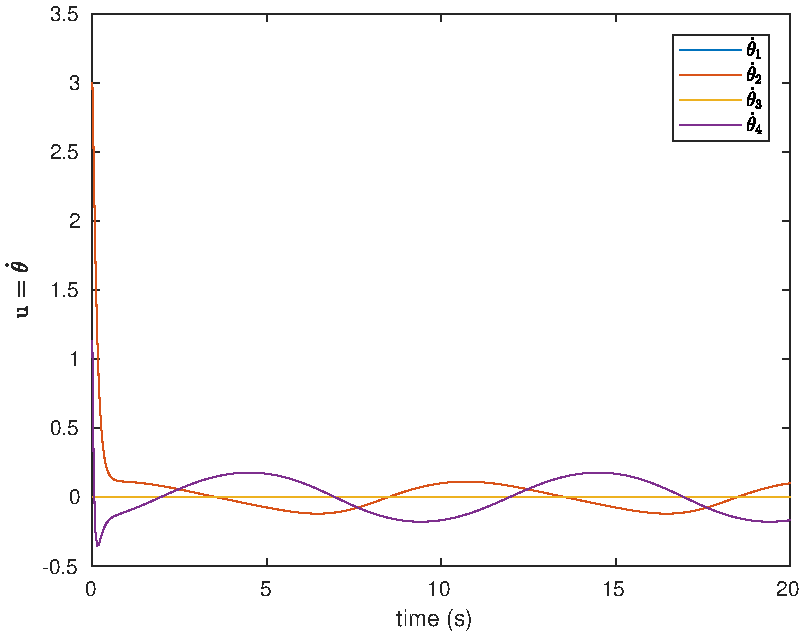
\includegraphics[width=1\textwidth]{figs/ex1_b_2_dq.pdf}
    \caption{$u = \dot{\theta}$}
    \label{fig:ex1_b_2_dq}
    \end{subfigure}
  \end{minipage}
\caption{Ex 1: Trajetória $b$, controle sem FF.}
\label{fig:ex1_b_2}
\end{figure}


\begin{figure}[!ht]
\centering
  \begin{minipage}{\linewidth}
  \centering
    \begin{subfigure}[b]{0.4\textwidth}
    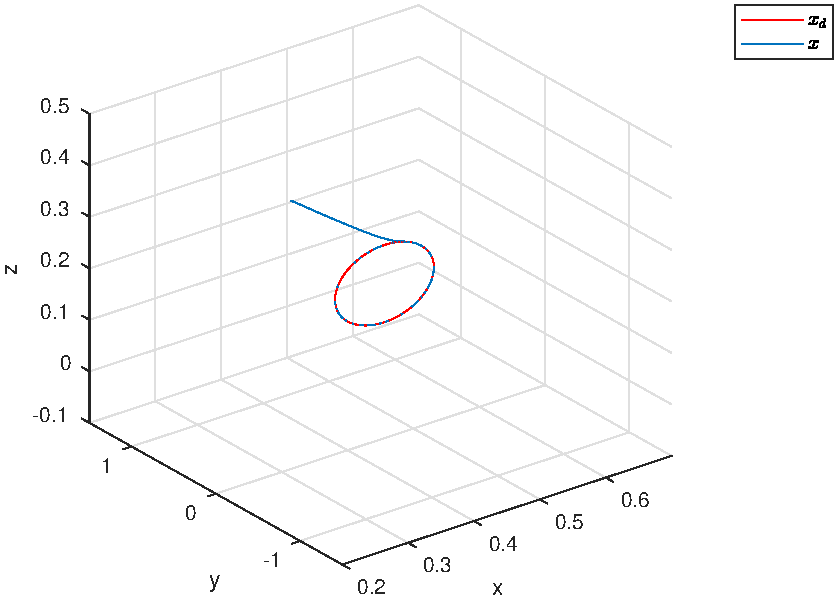
\includegraphics[width=1\textwidth]{figs/ex1_b_1_x.pdf}
    \caption{$x_d$ e $x$}
    \label{fig:ex1_b_1_x}
    \end{subfigure}
  \end{minipage}
  \begin{minipage}{\linewidth}
  \centering
    \begin{subfigure}[b]{0.4\textwidth}
    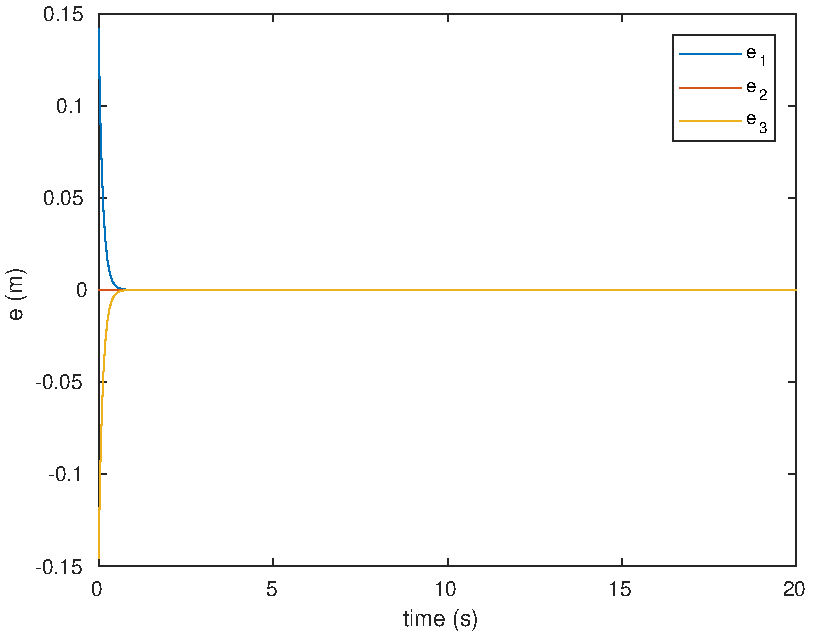
\includegraphics[width=1\textwidth]{figs/ex1_b_1_e.pdf}
    \caption{$e = x_d - x$}
    \label{fig:ex1_b_1_e}
    \end{subfigure}
    \begin{subfigure}[b]{0.4\textwidth}
    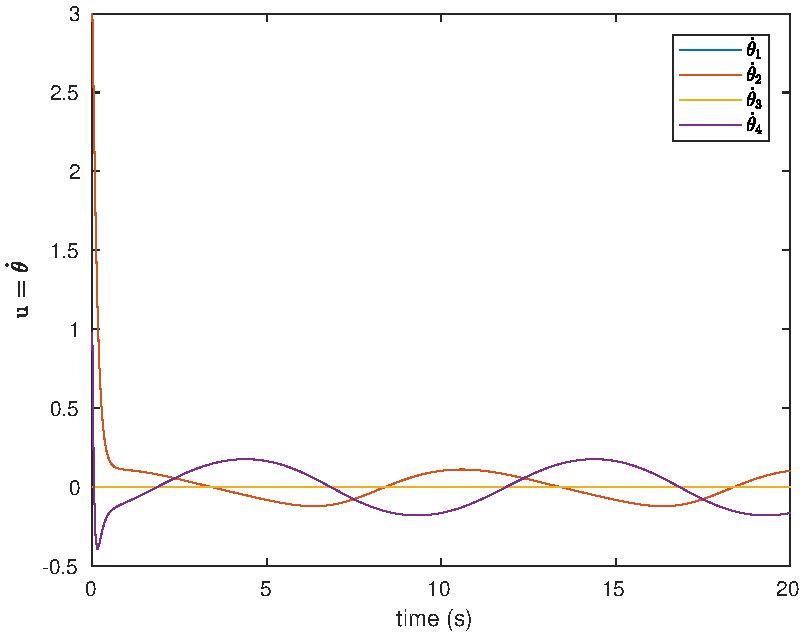
\includegraphics[width=1\textwidth]{figs/ex1_b_1_dq.pdf}
    \caption{$u = \dot{\theta}$}
    \label{fig:ex1_b_1_dq}
    \end{subfigure}
  \end{minipage}
\caption{Ex 1: Trajetória $b$, controle com FF.}
\label{fig:ex1_b_1}
\end{figure}


\begin{figure}[!ht]
\centering
  \begin{minipage}{\linewidth}
  \centering
    \begin{subfigure}[b]{0.4\textwidth}
    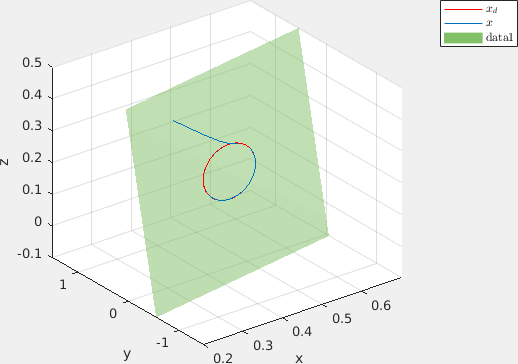
\includegraphics[width=1\textwidth]{figs/ex1_c_2_x.png}
    \caption{$x_d$ e $x$}
    \label{fig:ex1_c_2_x}
    \end{subfigure}
  \end{minipage}
  \begin{minipage}{\linewidth}
  \centering
    \begin{subfigure}[b]{0.4\textwidth}
    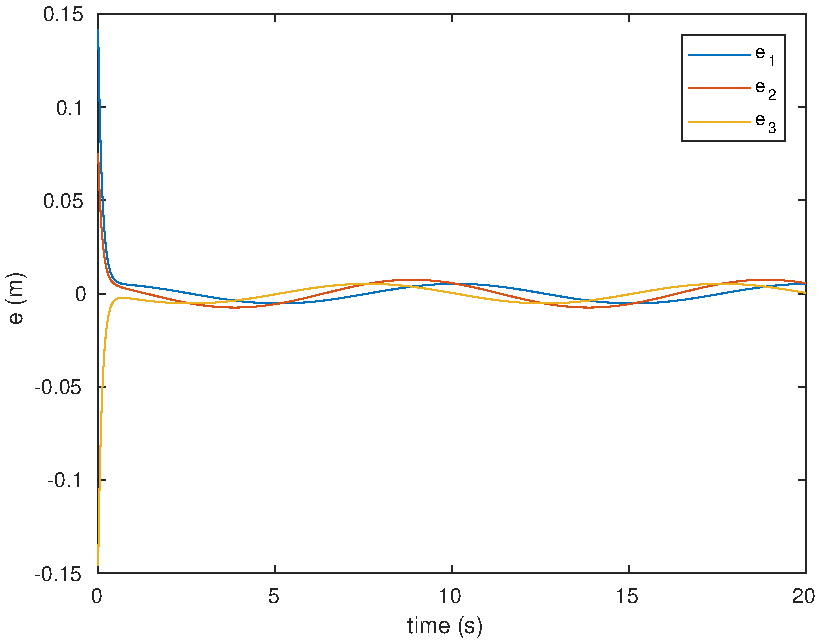
\includegraphics[width=1\textwidth]{figs/ex1_c_2_e.pdf}
    \caption{$e = x_d - x$}
    \label{fig:ex1_c_2_e}
    \end{subfigure}
    \begin{subfigure}[b]{0.4\textwidth}
    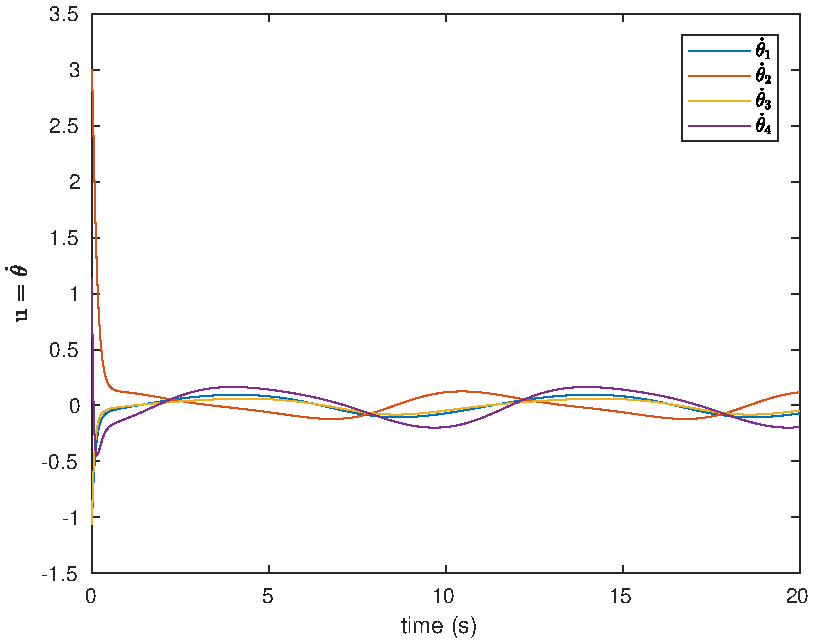
\includegraphics[width=1\textwidth]{figs/ex1_c_2_dq.pdf}
    \caption{$u = \dot{\theta}$}
    \label{fig:ex1_c_2_dq}
    \end{subfigure}
  \end{minipage}
\caption{Ex 1: Trajetória $c$, controle sem FF.}
\label{fig:ex1_c_2}
\end{figure}


\begin{figure}[!ht]
\centering
  \begin{minipage}{\linewidth}
  \centering
    \begin{subfigure}[b]{0.4\textwidth}
    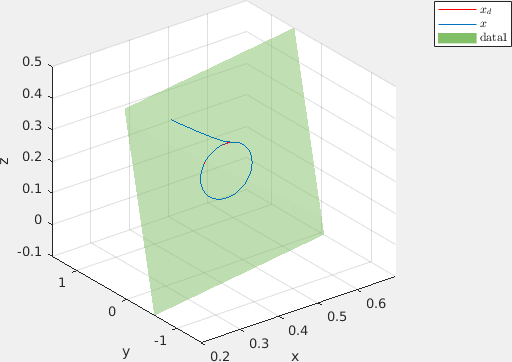
\includegraphics[width=1\textwidth]{figs/ex1_c_1_x.png}
    \caption{$x_d$ e $x$}
    \label{fig:ex1_c_1_x}
    \end{subfigure}
  \end{minipage}
  \begin{minipage}{\linewidth}
  \centering
    \begin{subfigure}[b]{0.4\textwidth}
    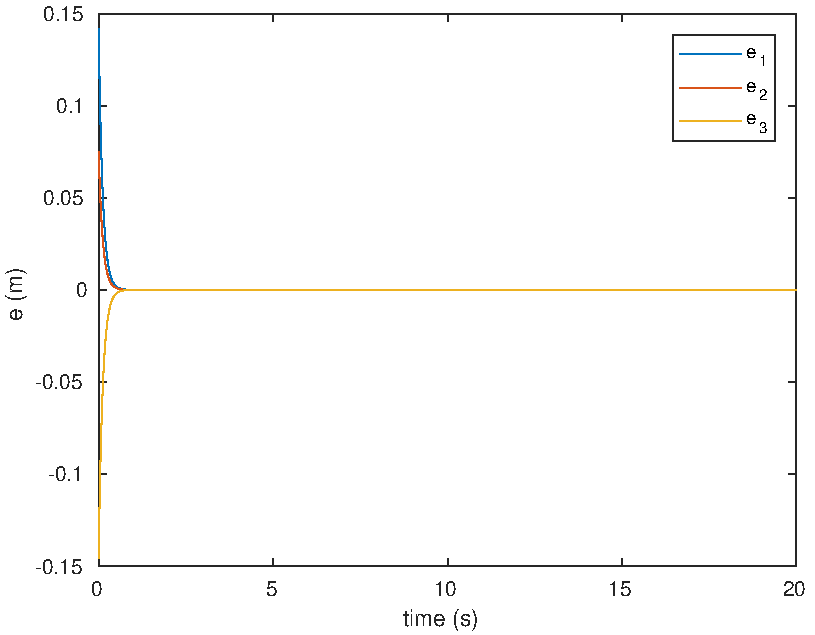
\includegraphics[width=1\textwidth]{figs/ex1_c_1_e.pdf}
    \caption{$e = x_d - x$}
    \label{fig:ex1_c_1_e}
    \end{subfigure}
    \begin{subfigure}[b]{0.4\textwidth}
    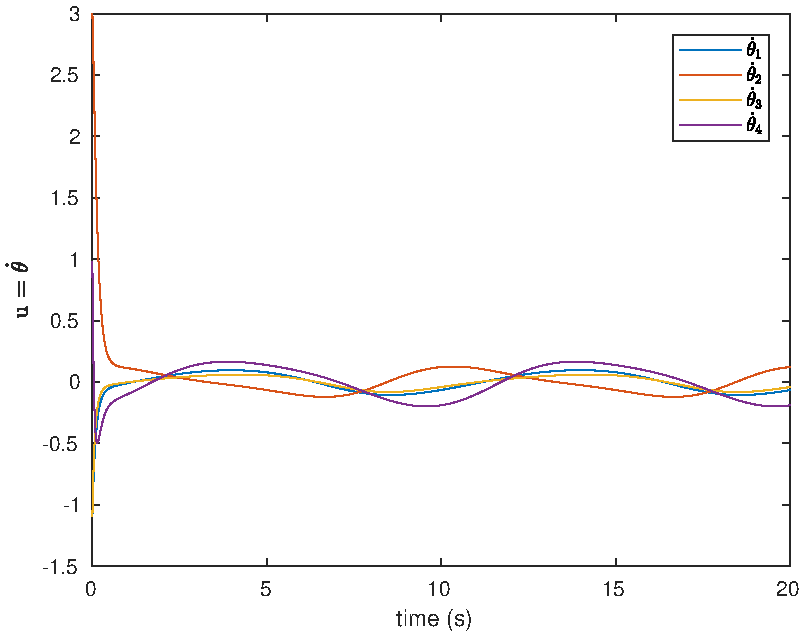
\includegraphics[width=1\textwidth]{figs/ex1_c_1_dq.pdf}
    \caption{$u = \dot{\theta}$}
    \label{fig:ex1_c_1_dq}
    \end{subfigure}
  \end{minipage}
\caption{Ex 1: Trajetória $c$, controle com FF.}
\label{fig:ex1_c_1}
\end{figure}


\section{Controle Cinemático de Manipuladores Redundantes} % 1

Diferente do manipulador anterior, o objetivo agora é controlar um manipulador redundante. Onde o Jacobiano perde posto por ter mais juntas do que graus de liberdade para a tarefa. 

Nesse caso aparece um comportamento muito interessante, o espaço nulo do Jacobiano, que permite otimizar um grau de liberdade adicional.

A função objetivo a ser otimizada pode ser de diversos tipos. Nesse trabalho, as escolhidas serão a \textbf{orientação},  a \textbf{manipulabilidade} e o \textbf{limite das juntas}.

O manipulador proposto para estudar esse comportamento é o manipulador planar 3R, com comprimento dos 3 elos de $0.5m$.

Assim como foi feito para o manipulador anterior, é necessário utilizar o método de Denavit-Hartenberg, cujos parâmetros estão na tabela \ref{tab:ex2_dh}.

A posição inicial escolhida foi $ q_0 = [\pi, -\pi/2, -\pi/2]^T $, representada na figura \ref{fig:ex2_ready}.

Neste caso, a trajetória desejada é um círculo de raio $0.25m$ com centro no ponto $[0.25 0.5]$. Parametrizada por $x_d$.


   	\begin{gather*}
	x_{d} = 
	\begin{bmatrix} 
	0.25 (1 - cos(\pi t)) \\ 
	0.25 (2 + sin(\pi t)) \\
	\end{bmatrix} \qquad t \in [0,4] \\
	\end{gather*}


\begin{table}[!ht]
\centering
\caption{Tabela de Denavit-Hartenberg do Manipulador Planar 3R.}
\label{tab:ex2_dh}

\begin{tabular}{|c|c|c|c|c|c|}
\hline
Junta  & $\alpha (rad)$ & $A (m)$ & $\theta (rad)$ & $D (m)$ & $Offset (rad)$ \\ \hline
$1$  & 0 & $0.5$ & $\theta_1$ & 0 & 0 \\ \hline
$2$  & 0 & $0.5$ & $\theta_2$ & 0 & 0 \\ \hline
$3$  & 0 & $0.5$ & $\theta_3$ & 0 & 0 \\ \hline

\end{tabular}
\end{table}

\begin{figure}[!ht]
\centering
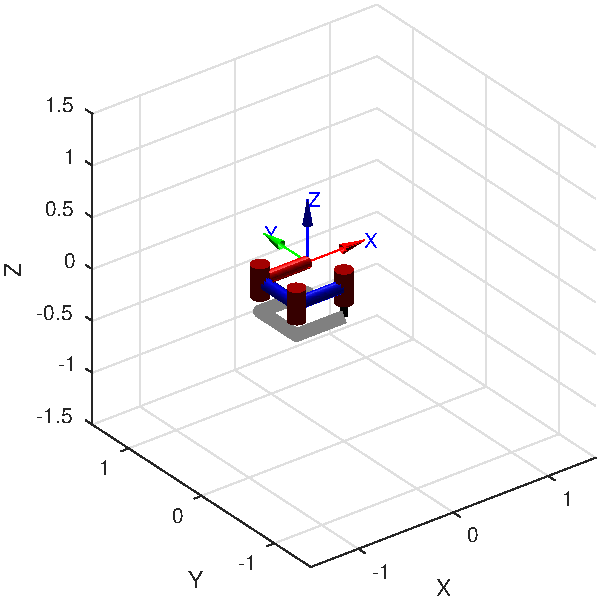
\includegraphics[width=0.5\textwidth]{figs/ex2_planar_tetha0.pdf}
\caption{Manipulador Planar 3R na posição inicial}
\label{fig:ex2_ready}
\end{figure}

\subsection{Controle}

Este caso é caracterizado por o numero de juntas $n$ ser maior do que o número de graus de liberdade da tarefa $m$. O que traria a necessidade de usar novamente a pseudo-inversa.

Porém, diferente do caso anterior, esse tem outra particularidade. Como o manipulador é planar com todas as juntas de rotação no eixo $z$, duas linhas do Jacobiano serão nulas. Além disso, por todas as juntas estarem em todo o tempo no plano XY, a terceira linha do Jacobiano, referente a posição no eixo $z$, também será zero.

Com isso, pode-se trabalhar com um Jacobiano reduzido chamado de Jacobiano Analítico ($J_a \in R^{3x3}$). Por $J_a$ ser quadrado e não singular, ele é inversível.

Ao reduzir o Jacobiano, também se faz necessário reduzir o sinal de controle ($u \in R^{6}$), passando a ter dimensão 3.


\subsubsection{Orientação}

No primeiro caso de controle, pede-se para que a orientação também siga uma trajetória desejada ($\phi_d$).

\begin{gather*}
	u = \dot{\theta} \qquad J_a \in R^{3x3} \\
	\dot{x} = J_a(\theta)\dot{\theta} = J_a(\theta)u \quad \Rightarrow \quad
	u = J_a(\theta)^{-1}\dot{x} \\
	u = J_a(\theta)^{-1} \bar{u} \\
	\bar{u} = \dot{x_d} + K (x_d - x) \\
	x_d = 
	\begin{bmatrix} 
	p_d \\ 
	\phi_d \\
	\end{bmatrix} \\
	p_{d} = 
	\begin{bmatrix} 
	0.25 (1 - cos(\pi t)) \\ 
	0.25 (2 + sin(\pi t)) \\
	0 \\
	\end{bmatrix}, \qquad 
	\phi_{d} = 
	\begin{bmatrix} 
	0 \\ 
	0 \\
	sin(\pi t / 24) \\
	\end{bmatrix} \quad \Rightarrow \quad 
	\dot{\phi_d} = 
	\begin{bmatrix} 
	0 \\
	0 \\
	\dfrac{\pi cos(\pi t / 24)}{24} \\
	\end{bmatrix} \qquad t \in [0,4] \\
	x_d = 
	\begin{bmatrix} 
	x \\ 
	y \\
	z \\
	\phi_1 \\
	\phi_2 \\
	\phi_3 \\
	\end{bmatrix}, \quad
	x_d = 
	\begin{bmatrix} 
	x \\ 
	y \\
	0 \\
	0 \\
	0 \\
	\phi_3 \\
	\end{bmatrix}
\end{gather*}

Para se controlar o sistema com 3 graus de liberdade, adiciona-se uma nova parcela no sintal de controle, o espaço nulo do Jacobiano, que é alcançado usando-se a pseudo-inversa dele. A variável $\mu$, o grau de liberdade adicional, é calculada multiplicando-se um ganho $K_0$ pela derivada da função $\omega(\theta)$ a ser otimizada.

Isso não altera a equação do erro.

\begin{gather*}
	\bar{u} = J^{\dagger}[\dot{x_d} + K(x_d - x)] + (I - J^{\dagger}J)\mu \\
	\dot{e} + Ke = 0 \\
	\mu = K_0\left( \dfrac{\partial \omega(\theta)}{\partial \theta} \right)^T  \\
	\omega(\theta) = 
	\begin{bmatrix} 
	0 \\
	0 \\
	sin(\pi t / 24) \\
	\end{bmatrix}
\end{gather*}
\begin{gather*}
	\phi_d = \theta_1 + \theta_2 + \theta_3 = sin(\pi t / 24) \\
	\omega(\theta) = 
	\begin{bmatrix} 
	0 \\
	0 \\
	sin(\pi t / 24) \\
	\end{bmatrix} \quad \Rightarrow \quad 
	\dot{\omega}(\theta) = 
	\begin{bmatrix} 
	0 \\
	0 \\
	\dfrac{\pi cos(\pi t / 24)}{24} \\
	\end{bmatrix}
\end{gather*}
 
\subsection{Funções Objetivo}

\subsubsection{Orientação}

Como observado anteriormente, uma das funções a ser otimizada é a orientação, que deve seguir uma trajetória parametrizada por $\phi_d$.

\begin{gather*}
	\phi_d = \theta_1 + \theta_2 + \theta_3 = sin(\pi t / 24) \\
	\omega(\theta) = 
	\begin{bmatrix} 
	0 \\
	0 \\
	sin(\pi t / 24) \\
	\end{bmatrix} \quad \Rightarrow \quad 
	\dot{\omega}(\theta) = 
	\begin{bmatrix} 
	0 \\
	0 \\
	\dfrac{\pi cos(\pi t / 24)}{24} \\
	\end{bmatrix}
\end{gather*}

\end{document}
